\documentclass[11pt,a4paper]{article}

\usepackage[margin=2.45cm]{geometry}
\usepackage{amsmath,amssymb,amsthm,mathtools}
\usepackage{booktabs,longtable,array}
\usepackage{enumitem}
\usepackage{microtype}
\usepackage{xcolor}
\usepackage{tikz}
\usepackage{pgfplots}
\pgfplotsset{compat=1.18}
\usepackage{hyperref}

\hypersetup{
  colorlinks=true,
  linkcolor=blue,
  citecolor=blue,
  urlcolor=blue,
  pdftitle={A Geometry-Dependent Generalization of the Diocotron Benchmark}
}

\newcommand{\R}{\mathbb{R}}
\newcommand{\C}{\mathbb{C}}
\newcommand{\Om}{\Omega}
\newcommand{\dd}{\,\mathrm{d}}
\newcommand{\bracket}[2]{\left\{#1,#2\right\}}
\newcommand{\norm}[1]{\left\|#1\right\|}
\newcommand{\abs}[1]{\left|#1\right|}
\newcommand{\ip}[2]{\left\langle #1,#2\right\rangle}
\newcommand{\G}{\mathcal{G}_{\Om}}
\newcommand{\Lop}{\mathcal{L}_{\star}}
\newcommand{\Torus}{\mathbb{S}^{1}}
\newcommand{\e}{\mathrm{e}}

\newtheorem{definition}{Definition}[section]
\newtheorem{remark}{Remark}[section]
\newtheorem{proposition}{Proposition}[section]

\title{\textbf{A Geometry-Dependent Generalization of the Diocotron Benchmark}\\[0.4em]
\large Equilibria, intrinsic perturbations, spectral references, and corner-sensitive tests}
\author{}
\date{}

\begin{document}

\maketitle

\begin{abstract}
The classical diocotron test on a disk is unusually complete: rotational symmetry supplies a radial equilibrium, a canonical angular variable, a Fourier decomposition, and an analytical dispersion relation. A change of mesh or boundary shape destroys this structure. The appropriate generalization is therefore not merely to place the same initial density on a noncircular mesh, but to reconstruct the equilibrium, perturbation coordinates, observables, and reference linear dynamics intrinsically from the domain.

This document proposes such a construction for the two-dimensional guiding-center model on bounded simply connected domains. Torsion-function level sets are retained as a robust mechanism for selecting and initializing a localized band. After convergence of the semilinear equilibrium, however, the dynamically natural coordinates are action--angle coordinates associated with the equilibrium stream function. They reduce exactly to polar action--angle coordinates on the disk, preserve the area measure, and make it possible to define both disk-like Fourier perturbations and exactly isovortical interface displacements. The linearized problem is then formulated as a nonlocal, generally nonnormal eigenvalue problem. On noncircular domains a prescribed harmonic is no longer generally an eigenmode, so two different tests are required: an eigenmode growth-rate test and a disk-analogue response test. Smooth shape deformations can be treated by spectral continuation and shape derivatives, whereas divertor-like domains with reentrant corners require corner-aware reference computations and a separate equilibrium-preservation protocol.
\end{abstract}

\tableofcontents

\section{Guiding-center model and Hamiltonian structure}

Let $\Om\subset\R^2$ be bounded and simply connected. For the smooth-domain discussion, assume initially that $\partial\Om$ is of class $C^{2,\alpha}$. Polygonal and cornered domains are treated separately in Section~\ref{sec:corners}. The guiding-center model is
\begin{align}
  \partial_t\rho+\bracket{\phi}{\rho}&=0
  &&\text{in }(0,T)\times\Om, \label{eq:transport}\\
  -\Delta\phi&=\rho
  &&\text{in }\Om, \label{eq:poisson}\\
  \phi&=0
  &&\text{on }\partial\Om. \label{eq:dirichlet}
\end{align}
The Poisson bracket is
\[
  \bracket{f}{g}
  :=
  \partial_xf\,\partial_yg-
  \partial_yf\,\partial_xg,
\]
and the incompressible velocity is
\[
  \mathbf{u}=\nabla^\perp\phi:=(-\partial_y\phi,\partial_x\phi).
\]
Thus
\[
  \bracket{\phi}{\rho}=\mathbf{u}\cdot\nabla\rho,
  \qquad
  \nabla\cdot\mathbf{u}=0,
  \qquad
  \mathbf{u}\cdot\mathbf{n}=0\quad\text{on }\partial\Om.
\]

Let
\[
  \G:=(-\Delta_D)^{-1}
\]
denote the inverse Dirichlet Laplacian, so that $\phi=\G\rho$. Equation~\eqref{eq:transport} is then the active-scalar equation
\begin{equation}
  \partial_t\rho+\bracket{\G\rho}{\rho}=0.
  \label{eq:active-scalar}
\end{equation}

For sufficiently regular solutions, the model preserves the mass
\begin{equation}
  \mathcal{M}(\rho)=\int_\Om\rho\,\dd x,
  \label{eq:mass}
\end{equation}
the energy
\begin{equation}
  \mathcal{E}(\rho)
  =\frac12\int_\Om\rho\,\G\rho\,\dd x
  =\frac12\int_\Om\abs{\nabla\phi}^2\,\dd x,
  \label{eq:energy}
\end{equation}
and every Casimir
\begin{equation}
  \mathcal{C}_{\Gamma}(\rho)
  =\int_\Om\Gamma(\rho)\,\dd x,
  \label{eq:casimir}
\end{equation}
for suitable scalar functions $\Gamma$. These invariants are central to the benchmark because instability growth should occur without artificial change of the transported vorticity distribution.

On a disk, rotational invariance yields an additional angular-impulse invariant. A generic domain has no continuous rotational symmetry and therefore no corresponding invariant. This is not a numerical defect: the list of physically relevant invariants is itself geometry dependent. Discrete reflection or rotational symmetries can still be used to decompose the linearized problem into symmetry classes, but they do not generally generate additional scalar conservation laws.

\section{Exact equilibria and torsion-based initialization}

\subsection{Steady-state condition}

A steady state $(\rho_\star,\phi_\star)$ satisfies
\begin{equation}
  \bracket{\phi_\star}{\rho_\star}=0,
  \qquad
  -\Delta\phi_\star=\rho_\star,
  \qquad
  \phi_\star|_{\partial\Om}=0.
  \label{eq:steady-general}
\end{equation}
A sufficient and structurally natural condition is
\begin{equation}
  \rho_\star=F(\phi_\star),
  \label{eq:rho-F-phi}
\end{equation}
which reduces the equilibrium computation to the semilinear Dirichlet problem
\begin{equation}
  -\Delta\phi_\star=F(\phi_\star)
  \quad\text{in }\Om,
  \qquad
  \phi_\star=0
  \quad\text{on }\partial\Om.
  \label{eq:semilinear}
\end{equation}
\subsubsection{Logistic window profile}

We use the standard logistic function
\begin{equation}
  \sigma(z)
  :=\frac{1}{1+\exp(-z)},
  \qquad z\in\R.
  \label{eq:logistic-function}
\end{equation}
It satisfies
\begin{equation}
  \sigma'(z)=\sigma(z)\bigl(1-\sigma(z)\bigr),
  \qquad
  \lim_{z\to-\infty}\sigma(z)=0,
  \qquad
  \lim_{z\to+\infty}\sigma(z)=1.
  \label{eq:logistic-properties}
\end{equation}
For two levels $a<b$ and a smoothing thickness $\delta>0$, define the smooth window
\begin{equation}
  W_{a,b,\delta}(s)
  :=
  \sigma\!\left(\frac{s-a}{\delta}\right)
  -
  \sigma\!\left(\frac{s-b}{\delta}\right).
  \label{eq:logistic-window-definition}
\end{equation}
For $s$ well inside $(a,b)$, one has $W_{a,b,\delta}(s)\simeq1$, whereas the window is exponentially small outside this interval. Moreover,
\begin{equation}
  W_{a,b,\delta}(s)
  \longrightarrow \mathbf{1}_{(a,b)}(s)
  \qquad\text{as }\delta\to0^+,
  \label{eq:logistic-sharp-limit}
\end{equation}
for every $s\notin\{a,b\}$. Its derivative is
\begin{align}
  W'_{a,b,\delta}(s)
  =\frac{1}{\delta}\Bigg[
  &\sigma\!\left(\frac{s-a}{\delta}\right)
   \left(1-\sigma\!\left(\frac{s-a}{\delta}\right)\right)
  \nonumber\\
  &-
  \sigma\!\left(\frac{s-b}{\delta}\right)
   \left(1-\sigma\!\left(\frac{s-b}{\delta}\right)\right)
  \Bigg].
  \label{eq:logistic-window-derivative}
\end{align}
Thus $W'_{a,b,\delta}$ is concentrated in two transition layers of thickness $O(\delta)$, with opposite signs at the two edges.

The equilibrium constitutive law used in the project is therefore
\begin{equation}
  F(z)
  =\rho_{\max}W_{c_-,c_+,\delta}(z)
  =\rho_{\max}
  \left[
    \sigma\!\left(\frac{z-c_-}{\delta}\right)
    -
    \sigma\!\left(\frac{z-c_+}{\delta}\right)
  \right],
  \qquad c_-<c_+.
  \label{eq:F-window}
\end{equation}
The derivative $F'$ changes sign across the two transition layers, reflecting the two interacting edges of the band.

\begin{figure}[ht]
  \centering
  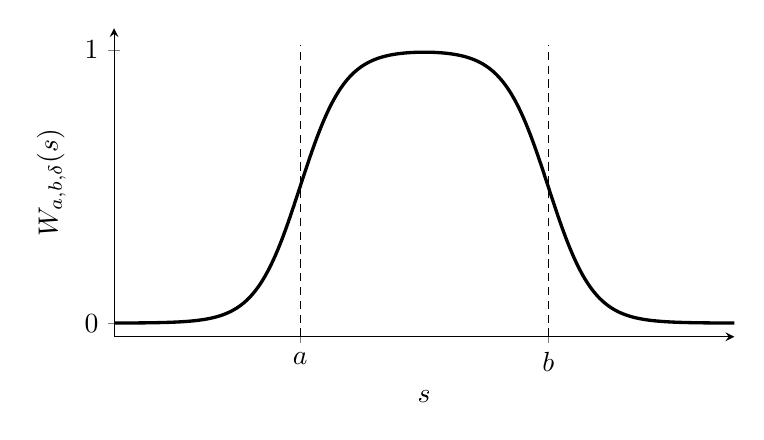
\begin{tikzpicture}
    \begin{axis}[
      width=0.78\textwidth,
      height=5.5cm,
      axis lines=left,
      xmin=-0.5,
      xmax=4.5,
      ymin=-0.05,
      ymax=1.08,
      xlabel={$s$},
      ylabel={$W_{a,b,\delta}(s)$},
      xtick={1,3},
      xticklabels={$a$,$b$},
      ytick={0,1},
      samples=350,
      domain=-0.5:4.5,
      clip=false
    ]
      \addplot[very thick]
      {
        1/(1+exp(-(x-1)/0.18))
        -
        1/(1+exp(-(x-3)/0.18))
      };
      \addplot[densely dashed] coordinates {(1,-0.05) (1,1.02)};
      \addplot[densely dashed] coordinates {(3,-0.05) (3,1.02)};
    \end{axis}
  \end{tikzpicture}
  \caption{Logistic window $W_{a,b,\delta}$ with $a=1$, $b=3$, and $\delta=0.18$. The smoothing parameter controls the thickness of the two transition layers.}
  \label{fig:logistic-window}
\end{figure}

Equation~\eqref{eq:rho-F-phi} is stronger than merely asking that the initial density look annular. It guarantees that vorticity contours and streamlines coincide. This exact compatibility is essential when the aim is to measure small linear growth rates.

\subsection{Torsion field as a geometric initializer}

Let the torsion function $\tau$ solve
\begin{equation}
  -\Delta\tau=1
  \quad\text{in }\Om,
  \qquad
  \tau=0
  \quad\text{on }\partial\Om.
  \label{eq:torsion}
\end{equation}
Choose regular values $\tau_-<\tau_+$ and define the torsion band
\begin{equation}
  B_{\tau}
  =\left\{x\in\Om:\tau_-\leq\tau(x)\leq\tau_+\right\}.
  \label{eq:torsion-band}
\end{equation}
The regular-band condition is
\begin{equation}
  \inf_{x\in B_\tau}\abs{\nabla\tau(x)}>0.
  \label{eq:regular-torsion-band}
\end{equation}
It ensures that the selected level sets form a smooth nested family and that $B_\tau$ is topologically an annulus.

The torsion profile provides a geometry-sensitive initial guess, for example
\begin{equation}
  \rho_{\mathrm{tor}}(x)
  =\rho_{\max}
  \left[
    \sigma\!\left(\frac{\tau(x)-\tau_-}{\delta_\tau}\right)
    -
    \sigma\!\left(\frac{\tau(x)-\tau_+}{\delta_\tau}\right)
  \right].
  \label{eq:raw-torsion-profile}
\end{equation}
However, $\rho_{\mathrm{tor}}$ is not in general an exact equilibrium of~\eqref{eq:transport}--\eqref{eq:dirichlet}. It should therefore be used to initialize a continuation/Newton solve for~\eqref{eq:semilinear}, not as the final reference state for growth-rate measurements.

\begin{remark}[Two distinct benchmark states]
The benchmark should retain both the raw torsion-window state and the converged semilinear state:
\begin{enumerate}[label=(\roman*)]
  \item the raw state measures the quality of the equilibrium-construction procedure;
  \item the converged state measures the fidelity of the time-dependent scheme to the true linearized dynamics.
\end{enumerate}
Conflating these two tests makes it impossible to determine whether observed growth comes from physical instability or from an inaccurate initial equilibrium.
\end{remark}

\section{Regular equilibrium bands and intrinsic action--angle coordinates}
\label{sec:action-angle}

The torsion field is used to construct and position the initial band. Once the semilinear equilibrium has converged, however, the dynamically natural coordinates must be constructed from the equilibrium stream function $\phi_\star$, because the equilibrium velocity
\begin{equation}
  X_\star:=\nabla^\perp\phi_\star
  \label{eq:equilibrium-vector-field}
\end{equation}
is tangent to the level sets of $\phi_\star$. This distinction is essential: torsion coordinates are geometric initialization coordinates, whereas equilibrium action--angle coordinates are canonical coordinates for the actual steady flow.

\subsection{Regular annular foliation of the equilibrium}

Choose two regular values $h_-<h_+$ in the range of $\phi_\star$ and define
\begin{equation}
  B_\star
  :=\left\{x\in\Om:h_-<\phi_\star(x)<h_+\right\}.
  \label{eq:equilibrium-band}
\end{equation}
Assume that
\begin{equation}
  \inf_{x\in\overline{B_\star}}\abs{\nabla\phi_\star(x)}>0,
  \label{eq:regular-equilibrium-band}
\end{equation}
and that, for every $h\in[h_-,h_+]$, the level set
\begin{equation}
  \Sigma_h:=\left\{x\in\Om:\phi_\star(x)=h\right\}
  \label{eq:equilibrium-level-set}
\end{equation}
is a smooth simple closed curve. We also assume that these curves are nested, so that $B_\star$ is diffeomorphic to an annulus.

Since
\begin{equation}
  X_\star\cdot\nabla\phi_\star=0,
\end{equation}
the integral curves of $X_\star$ are precisely the level curves $\Sigma_h$. Moreover,
\begin{equation}
  \abs{X_\star}=\abs{\nabla\phi_\star}.
\end{equation}
The time required for one complete orbit along $\Sigma_h$ is therefore
\begin{equation}
  T(h)
  :=\oint_{\Sigma_h}\frac{\dd\ell}{\abs{\nabla\phi_\star}}.
  \label{eq:period}
\end{equation}
Condition~\eqref{eq:regular-equilibrium-band} excludes stagnation points and guarantees that $T(h)$ is finite. If a critical level is crossed or the topology of the level sets changes, a single global action--angle system does not exist; such cases should be treated as a separate critical-level stress-test family.

\subsection{The action variable}

Let $D_h$ denote the bounded region enclosed by the Jordan curve $\Sigma_h$, and let
\begin{equation}
  A(h):=\abs{D_h}
\end{equation}
be its area. The action variable is the enclosed area divided by $2\pi$:
\begin{equation}
  I(x)
  :=\mathcal{I}\bigl(\phi_\star(x)\bigr),
  \qquad
  \mathcal{I}(h):=\frac{A(h)}{2\pi}.
  \label{eq:action-def}
\end{equation}
Thus $I$ is constant on each equilibrium streamline and labels the nested streamlines by the area they enclose, rather than directly by the value of $\phi_\star$.

By the coarea formula,
\begin{equation}
  \abs{A'(h)}
  =\oint_{\Sigma_h}\frac{\dd\ell}{\abs{\nabla\phi_\star}}
  =T(h).
  \label{eq:area-period-relation}
\end{equation}
Because no critical level is crossed in $B_\star$, the sign of $A'(h)$ is constant. Define
\begin{equation}
  \varepsilon_{B}
  :=\operatorname{sign}A'(h)\in\{-1,+1\}.
  \label{eq:band-orientation}
\end{equation}
Then
\begin{equation}
  \frac{\dd\mathcal{I}}{\dd h}(h)
  =\varepsilon_B\frac{T(h)}{2\pi}.
  \label{eq:action-derivative}
\end{equation}
The sign $\varepsilon_B$ records whether the enclosed area increases or decreases as the stream-function level $h$ increases. Since $\mathcal I$ is strictly monotone, it can be inverted on the band. We write
\begin{equation}
  h=H(I).
  \label{eq:H-inverse-action}
\end{equation}
Differentiating the inverse relation gives the equilibrium angular frequency
\begin{equation}
  \Omega(I)
  :=H'(I)
  =\varepsilon_B\frac{2\pi}{T(H(I))}.
  \label{eq:orbital-frequency}
\end{equation}

The action has a direct geometric meaning. If $h_1$ and $h_2$ are two levels in the band, then
\begin{equation}
  2\pi\bigl(I(h_2)-I(h_1)\bigr)
  =A(h_2)-A(h_1),
  \label{eq:action-area-difference}
\end{equation}
so, up to orientation, an action difference is exactly the area enclosed between the corresponding equilibrium streamlines.

\subsection{The angle variable}

To define a phase along each closed streamline, choose a smooth transversal curve
\begin{equation}
  \Gamma_{\mathrm{cut}}\subset\overline{B_\star}
\end{equation}
that intersects each $\Sigma_h$ exactly once and transversely. Let
\begin{equation}
  p(h):=\Gamma_{\mathrm{cut}}\cap\Sigma_h
\end{equation}
be the reference point on the streamline $\Sigma_h$.

Let $\Phi_t^\star$ denote the flow generated by $X_\star$:
\begin{equation}
  \frac{\dd}{\dd t}\Phi_t^\star(x)
  =X_\star\bigl(\Phi_t^\star(x)\bigr),
  \qquad
  \Phi_0^\star(x)=x.
  \label{eq:equilibrium-flow-map}
\end{equation}
For $x\in\Sigma_h$, let $t_h(x)$ be the travel time, defined modulo $T(h)$, such that
\begin{equation}
  x=\Phi_{t_h(x)}^\star\bigl(p(h)\bigr).
\end{equation}
The angle variable is then
\begin{equation}
  \theta(x)
  :=\varepsilon_B\frac{2\pi t_h(x)}{T(h)}
  \quad\operatorname{mod}2\pi,
  \qquad h=\phi_\star(x).
  \label{eq:angle-def}
\end{equation}
Consequently, $\theta=0$ on the transversal and one complete orbit changes the unwrapped angle by $2\pi$.

Because $t_h$ is the physical travel time of the equilibrium velocity,
\begin{equation}
  X_\star\cdot\nabla\theta
  =\bracket{\phi_\star}{\theta}
  =\varepsilon_B\frac{2\pi}{T(\phi_\star)}.
  \label{eq:angle-transport}
\end{equation}
Equivalently, $\theta$ solves the transport problem
\begin{equation}
  \nabla^\perp\phi_\star\cdot\nabla\theta
  =\varepsilon_B\frac{2\pi}{T(\phi_\star)}
  \quad\text{in }B_\star,
  \qquad
  \theta\big|_{\Gamma_{\mathrm{cut}}}=0,
  \label{eq:angle-pde}
\end{equation}
with a $2\pi$ jump across the branch cut $\Gamma_{\mathrm{cut}}$.

The angle $\theta$ is not generally a Euclidean polar angle or a normalized arc-length coordinate. Equal increments of $\theta$ represent equal fractions of the equilibrium travel time. Hence regions in which $\abs{\nabla\phi_\star}$ is small occupy a larger arc-length interval for a given phase increment, while regions of large equilibrium speed occupy a smaller one.

\subsection{Canonical relation and area preservation}

Since $I=\mathcal I(\phi_\star)$, the chain rule gives
\begin{equation}
  \bracket{I}{\theta}
  =\mathcal I'(\phi_\star)\bracket{\phi_\star}{\theta}.
\end{equation}
Using~\eqref{eq:action-derivative} and~\eqref{eq:angle-transport},
\begin{equation}
  \bracket{I}{\theta}
  =\left(\varepsilon_B\frac{T(\phi_\star)}{2\pi}\right)
   \left(\varepsilon_B\frac{2\pi}{T(\phi_\star)}\right)
  =1.
  \label{eq:canonical-relations}
\end{equation}
Thus $(I,\theta)$ are canonical coordinates on $B_\star$.

For sufficiently regular functions $f=f(I,\theta)$ and $g=g(I,\theta)$,
\begin{equation}
  \bracket{f}{g}
  =\partial_I f\,\partial_\theta g
   -\partial_\theta f\,\partial_I g.
  \label{eq:canonical-bracket}
\end{equation}
Moreover,
\begin{equation}
  \det\frac{\partial(I,\theta)}{\partial(x,y)}
  =\bracket{I}{\theta}=1,
\end{equation}
and therefore
\begin{equation}
  \dd x=\dd I\,\dd\theta.
  \label{eq:canonical-bracket-measure}
\end{equation}
This exact area-preservation identity is one of the principal advantages of the area-based action variable. In particular, no additional Jacobian factor appears when integrating over the band, and every nonzero Fourier harmonic in $\theta$ has exactly zero mean over the band.

\subsection{Equilibrium dynamics in action--angle form}

Since $I$ is a monotone function of $\phi_\star$ on the regular band, the equilibrium stream function and density can be written as
\begin{equation}
  \phi_\star=H(I),
  \qquad
  \rho_\star=F(\phi_\star)=\overline\rho(I),
  \qquad
  \overline\rho(I):=F(H(I)).
  \label{eq:equilibrium-action}
\end{equation}
For any scalar field $g$,
\begin{equation}
  \bracket{\phi_\star}{g}
  =\bracket{H(I)}{g}
  =\Omega(I)\partial_\theta g.
  \label{eq:equilibrium-advection-action-angle}
\end{equation}
Thus the equilibrium trajectories satisfy
\begin{equation}
  \dot I=0,
  \qquad
  \dot\theta=\Omega(I).
  \label{eq:action-angle-trajectories}
\end{equation}
The equilibrium is therefore one-dimensional in action even though the geometry is not rotationally symmetric.

For perturbations
\begin{equation}
  \rho=\rho_\star+\eta,
  \qquad
  \phi=\phi_\star+\psi,
  \qquad
  -\Delta\psi=\eta,
\end{equation}
the linearized transport equation takes the form
\begin{equation}
  \partial_t\eta
  +\Omega(I)\partial_\theta\eta
  -\overline\rho'(I)\partial_\theta\psi
  =0.
  \label{eq:linearized-action-angle-preview}
\end{equation}
The geometry is not eliminated by the coordinate change: it remains in the Dirichlet Poisson solution operator $\eta\mapsto\psi$. On the disk this operator is invariant under angular translations and Fourier modes decouple. On a general domain it is not translation invariant in $\theta$, and different angular harmonics are coupled.

\subsection{Exact reduction to the disk}

Suppose $\Om$ is a disk and $\phi_\star(x)=\Phi_\star(r)$ is radial, with no critical radius in the chosen band. The level curves are circles, so
\begin{equation}
  A=\pi r^2,
  \qquad
  I=\frac{A}{2\pi}=\frac{r^2}{2}.
  \label{eq:disk-action}
\end{equation}
Moreover,
\begin{equation}
  T(r)=\frac{2\pi r}{\abs{\Phi_\star'(r)}},
\end{equation}
and the angle~\eqref{eq:angle-def}, after fixing its origin, coincides with the ordinary polar angle up to the orientation already encoded by $\varepsilon_B$. The angular frequency is
\begin{equation}
  \Omega(I)=\frac{\Phi_\star'(r)}{r}.
  \label{eq:disk-angular-frequency}
\end{equation}
Hence
\begin{equation}
  (I,\theta)=\left(\frac{r^2}{2},\theta_{\mathrm{polar}}\right)
\end{equation}
on the disk, and a generalized harmonic
\begin{equation}
  A_m(I)\cos\bigl(m(\theta-\theta_0)\bigr)
\end{equation}
reduces exactly to the usual azimuthal perturbation.

\begin{remark}[Why travel-time angle is preferable to transported arc length]
A normalized arc-length coordinate along each level set is reproducible but does not, in general, make the equilibrium angular velocity constant along an orbit. In contrast, the travel-time angle satisfies
\begin{equation}
  \frac{\dd\theta}{\dd t}=\Omega(I),
\end{equation}
which depends on the streamline label $I$ but not on the phase $\theta$. This is the canonical form needed for linear stability analysis and for comparison with disk dispersion theory.
\end{remark}

\subsection{Gauge freedom and the physical meaning of phase}

The canonical relation does not uniquely determine the angle. For any sufficiently smooth function $\beta(I)$,
\begin{equation}
  \widetilde\theta=\theta+\beta(I)
\end{equation}
still satisfies $\bracket{I}{\widetilde\theta}=1$. This freedom corresponds to choosing a different phase origin on each streamline. The transversal $\Gamma_{\mathrm{cut}}$, together with the condition $\theta=0$ on it, fixes this gauge.

On the disk, changing the transversal by a rigid rotation has no physical consequence because the domain and equilibrium are rotationally invariant. On a general domain, the phase origin fixes the location of the perturbation relative to geometric features. Thus the phase $\theta_0$ in
\begin{equation}
  \cos\bigl(m(\theta-\theta_0)\bigr)
\end{equation}
is a physically relevant benchmark parameter. For reproducibility, the transversal should be selected by a geometry-based rule, such as a symmetry axis, a direction of extremal boundary radius, the deepest concavity, the point of closest wall approach, or a torsion-gradient trajectory passing through a distinguished boundary point.

\subsection{Numerical construction on an unstructured mesh}

A practical construction proceeds as follows:
\begin{enumerate}
  \item Compute the converged equilibrium $(\rho_{\star,h},\phi_{\star,h})$.
  \item Select an interval $[h_-,h_+]$ on which the discrete level curves are closed and $\abs{\nabla\phi_{\star,h}}\geq\gamma_{\min}>0$.
  \item Extract a family of level curves $\Sigma_{h_j,h}$.
  \item Compute the enclosed areas $A_h(h_j)$ and periods
  \begin{equation}
    T_h(h_j)\approx\oint_{\Sigma_{h_j,h}}
    \frac{\dd\ell}{\abs{\nabla\phi_{\star,h}}}.
  \end{equation}
  \item Define $I_h(h_j)=A_h(h_j)/(2\pi)$ and interpolate the monotone relation between $I_h$ and $h_j$.
  \item Choose a discrete transversal $\Gamma_{\mathrm{cut},h}$.
  \item Integrate the discrete equilibrium flow from the transversal along each level curve and normalize the travel time by $T_h(h_j)$.
  \item Interpolate the resulting phase information across the band.
\end{enumerate}

Because $\theta$ has a $2\pi$ jump across the branch cut, it is usually preferable to store
\begin{equation}
  z(x):=\exp\bigl(\mathrm{i}\theta(x)\bigr),
  \label{eq:complex-phase-field}
\end{equation}
or the pair $(\cos\theta,\sin\theta)$ rather than a discontinuous real-valued angle. Then
\begin{equation}
  \cos(m\theta)=\operatorname{Re}(z^m),
  \qquad
  \sin(m\theta)=\operatorname{Im}(z^m),
\end{equation}
without introducing a numerical discontinuity along the cut.

\subsection{Relation to the torsion construction}

The torsion function $\tau$ and equilibrium stream function $\phi_\star$ have complementary but different roles. The torsion function provides a geometry-dependent initialization and permits direct control of the initial band position, thickness, and wall distance. The equilibrium stream function provides the true invariant streamlines, orbital periods, canonical action, and dynamically normalized phase.

A phase coordinate transported across torsion level sets can be useful during initialization, but it is not generally canonical for the converged equilibrium and need not satisfy $\bracket{I}{\theta}=1$. Instability perturbations and modal observables should therefore be defined using the action--angle coordinates of $\phi_\star$ after the semilinear equilibrium has converged.

\section{Perturbations: disk analogues and dynamically accessible deformations}

A useful benchmark must distinguish between an easily prescribed density perturbation and a perturbation generated by an area-preserving rearrangement of the equilibrium.

\subsection{Additive disk-analogue harmonics}

The direct analogue of a disk mode is
\begin{equation}
  \delta\rho_m(I,\theta)
  =A(I)\cos(m\theta+\theta_0),
  \qquad m\in\mathbb{N}.
  \label{eq:additive-mode}
\end{equation}
The initial state is
\begin{equation}
  \rho_0=\rho_\star+\varepsilon\delta\rho_m.
  \label{eq:additive-initial-state}
\end{equation}
Because $\dd x=\dd I\dd\theta$,
\begin{equation}
  \int_{B_\star}\delta\rho_m\,\dd x=0
  \label{eq:exact-zero-mass}
\end{equation}
for every transverse amplitude $A(I)$. Moreover, for any smooth $\Gamma$,
\[
  \frac{\dd}{\dd\varepsilon}
  \mathcal{C}_\Gamma(\rho_\star+\varepsilon\delta\rho_m)
  \bigg|_{\varepsilon=0}
  =0,
\]
because $\Gamma'(\rho_\star)$ depends only on $I$. Thus the Casimir defect of the additive perturbation begins at order $\varepsilon^2$.

Natural choices are
\begin{equation}
  A(I)=\overline\rho(I),
  \qquad
  A(I)=\overline\rho'(I),
  \qquad
  A(I)=\chi_{\mathrm{band}}(I),
  \label{eq:amplitude-choices}
\end{equation}
where the second choice localizes the perturbation at the two density-gradient layers and is the closest analogue of interacting diocotron edge waves.

The phase origin $\theta_0$ is a gauge choice unless the geometry supplies a preferred direction. Therefore cross-geometry comparisons should use the complex mode magnitude rather than the sign or phase of a cosine coefficient.

\subsection{Exactly isovortical perturbations}

The strongest conservation-compatible perturbation is obtained by rearranging the equilibrium through an area-preserving map. Let $\chi\in C_c^\infty(B_\star)$ and let $\Phi_\varepsilon$ be the flow of
\begin{equation}
  \boldsymbol\xi=\nabla^\perp\chi,
  \qquad
  \frac{\dd}{\dd\varepsilon}\Phi_\varepsilon
  =\boldsymbol\xi\circ\Phi_\varepsilon,
  \qquad
  \Phi_0=\operatorname{Id}.
  \label{eq:area-preserving-flow}
\end{equation}
Since $\nabla\cdot\boldsymbol\xi=0$ and $\chi$ is supported away from the wall, $\Phi_\varepsilon$ preserves area and the boundary. Define
\begin{equation}
  \rho_\varepsilon
  =\rho_\star\circ\Phi_\varepsilon^{-1}.
  \label{eq:isovortical-state}
\end{equation}
Then
\begin{equation}
  \mathcal{C}_\Gamma(\rho_\varepsilon)
  =\mathcal{C}_\Gamma(\rho_\star)
  \label{eq:exact-casimir-preservation}
\end{equation}
for every $\Gamma$, at finite $\varepsilon$, not merely to first order.

The first variation is
\begin{equation}
  \delta\rho
  :=\frac{\dd\rho_\varepsilon}{\dd\varepsilon}\bigg|_{\varepsilon=0}
  =-\bracket{\chi}{\rho_\star}.
  \label{eq:isovortical-tangent}
\end{equation}
In action--angle coordinates, take
\begin{equation}
  \chi_m(I,\theta)
  =\frac{b(I)}{m}\sin(m\theta+\theta_0).
  \label{eq:chi-mode}
\end{equation}
Then
\begin{equation}
  \delta\rho_m
  =b(I)\overline\rho'(I)
   \cos(m\theta+\theta_0).
  \label{eq:isovortical-mode}
\end{equation}
Hence the familiar interface-weighted harmonic arises naturally as the tangent to an exactly area-preserving displacement of the equilibrium.

This construction is recommended as the primary perturbation for conservation studies. Any change in the initial Casimir distribution then comes from numerical projection or quadrature, not from the mathematical definition of the perturbation.

\subsection{Physical interface displacement}

The generator~\eqref{eq:chi-mode} also gives a precise physical displacement of the equilibrium interfaces. Along the deformation flow,
\begin{equation}
  \delta I
  =\bracket{\chi_m}{I}
  =-\partial_\theta\chi_m
  =-b(I)\cos(m\theta+\theta_0).
  \label{eq:action-displacement}
\end{equation}
The normal displacement of the level set $I=I_\pm$ is therefore
\begin{equation}
  \delta n_\pm(\theta)
  =\frac{\delta I}{\abs{\nabla I}}
  \bigg|_{I=I_\pm}.
  \label{eq:normal-displacement}
\end{equation}
To prescribe a uniform physical displacement amplitude $d_\pm$, choose
\begin{equation}
  b(I_\pm)=-d_\pm\abs{\nabla I}\big|_{I=I_\pm}.
  \label{eq:b-physical-displacement}
\end{equation}
Interpolating $b(I)$ between its values at the two interfaces produces:
\begin{enumerate}[label=(\roman*)]
  \item inner-interface displacement only;
  \item outer-interface displacement only;
  \item in-phase displacement of both interfaces;
  \item out-of-phase displacement of the two interfaces.
\end{enumerate}
These four cases are equivalent only in highly symmetric settings. Their splitting on a general geometry is itself a meaningful benchmark output.

\subsection{Geometry-native and localized perturbations}

The disk-like harmonic family should be complemented by perturbations that probe the actual domain:
\begin{enumerate}
  \item the dominant right eigenmode of the linearized operator;
  \item an optimal transient-growth perturbation obtained from a singular vector of the linear propagator;
  \item a localized isovortical bump, generated by a $\chi(I,\theta)$ localized near high curvature, minimum wall distance, or a divertor mouth;
  \item parity-selective perturbations on domains with reflection symmetry;
  \item perturbations repeated at equivalent physical locations on differently oriented meshes, to isolate grid-orientation bias.
\end{enumerate}
A localized perturbation should preferably be defined through $\chi$, not by adding a density bump, so that the vorticity distribution remains unchanged initially.

\section{The geometry-dependent linearized diocotron operator}

\subsection{Strong formal linearization}

Write
\[
  \rho=\rho_\star+\eta,
  \qquad
  \phi=\phi_\star+\psi,
  \qquad
  -\Delta\psi=\eta.
\]
Keeping terms linear in $\eta$ gives
\begin{equation}
  \partial_t\eta
  +\bracket{\phi_\star}{\eta}
  +\bracket{\psi}{\rho_\star}
  =0,
  \qquad
  \psi=\G\eta.
  \label{eq:linearized}
\end{equation}
Thus
\begin{equation}
  \partial_t\eta=\Lop\eta,
  \qquad
  \Lop\eta
  :=-\bracket{\phi_\star}{\eta}
     -\bracket{\G\eta}{\rho_\star}.
  \label{eq:linear-operator}
\end{equation}
On a smooth domain with sufficiently regular equilibrium, this can be viewed as a closed nonselfadjoint operator on an $L^2$-based space with an $H^1$-type domain. For numerical reference work, the mixed weak formulation below is more robust than relying on a pointwise strong form.

\subsection{Mixed weak eigenproblem}

Let
\[
  b(a;b,c):=\int_\Om\bracket{a}{b}\,c\,\dd x.
\]
The linear eigenproblem is: find $\lambda\in\C$ and $(\eta,\psi)\neq(0,0)$ such that
\begin{align}
  \lambda(\eta,v)
  +b(\phi_\star;\eta,v)
  +b(\psi;\rho_\star,v)&=0
  &&\forall v, \label{eq:weak-eigen-transport}\\
  (\nabla\psi,\nabla q)-(\eta,q)&=0
  &&\forall q\in H_0^1(\Om). \label{eq:weak-eigen-poisson}
\end{align}
The first term may also be integrated by parts using the skew-symmetry of incompressible advection. This is useful when $\eta$ is represented discontinuously or when a common weak residual is required across FE, DG, and FV methods.

After discretization, the block system has the generic form
\begin{align}
  \lambda M_\rho\boldsymbol\eta
  +C_\star\boldsymbol\eta
  +D_\star\boldsymbol\psi&=0, \label{eq:block1}\\
  K\boldsymbol\psi-B\boldsymbol\eta&=0. \label{eq:block2}
\end{align}
Eliminating $\boldsymbol\psi$ yields a generalized non-Hermitian eigenproblem
\begin{equation}
  L_h\boldsymbol\eta
  =\lambda M_\rho\boldsymbol\eta,
  \qquad
  L_h=-\left(C_\star+D_\star K^{-1}B\right).
  \label{eq:discrete-eigenproblem}
\end{equation}
The Poisson inverse should be applied through linear solves rather than explicitly formed.

\subsection{Action--angle form and the loss of Fourier decoupling}

Using~\eqref{eq:equilibrium-action} and~\eqref{eq:canonical-bracket-measure}, the linearized transport equation becomes
\begin{equation}
  \partial_t\eta
  +\Omega(I)\partial_\theta\eta
  -\overline\rho'(I)\partial_\theta\psi
  =0,
  \qquad
  -\Delta_\Om\psi=\eta.
  \label{eq:linear-action-angle}
\end{equation}
The entire dependence on the domain is now concentrated in:
\begin{enumerate}[label=(\roman*)]
  \item the equilibrium frequency $\Omega(I)$;
  \item the radial profile $\overline\rho(I)$;
  \item the Dirichlet Green operator expressed in $(I,\theta)$ coordinates.
\end{enumerate}
Indeed,
\begin{equation}
  \psi(I,\theta)
  =\int
  G_\Om\bigl(X(I,\theta),X(I',\theta')\bigr)
  \eta(I',\theta')\,
  \dd I'\dd\theta'.
  \label{eq:green-action-angle}
\end{equation}

On the disk, the kernel depends on $\theta-\theta'$ and every Fourier subspace
\[
  \left\{\widehat\eta_m(I)\e^{im\theta}\right\}
\]
is invariant. This yields an independent eigenproblem for each azimuthal mode $m$. On a general domain, the kernel depends separately on $\theta$ and $\theta'$. Consequently, a prescribed $m$ harmonic generally excites other harmonics, and the classical mode number is no longer a conserved label.

This observation leads to a fundamental distinction:
\begin{description}
  \item[Eigenmode benchmark:] initialize with a right eigenmode and compare one exponential growth rate.
  \item[Disk-analogue response benchmark:] initialize with $A(I)\cos(m\theta)$ and compare the complete linear response, including transfer to other harmonics.
\end{description}
Trying to assign a single ``growth rate of the $m$ mode'' to the second test can be misleading when the geometry strongly couples harmonics.

\subsection{Nonnormality}

The operator $\Lop$ is generally nonnormal. Let $v_j$ and $w_j$ denote right and left eigenvectors of the discrete pencil,
\begin{align}
  L_hv_j&=\lambda_jM_\rho v_j,\\
  w_j^\ast L_h&=\lambda_jw_j^\ast M_\rho,
\end{align}
normalized by
\begin{equation}
  w_i^\ast M_\rho v_j=\delta_{ij}.
  \label{eq:biorthogonality}
\end{equation}
The correct modal amplitude is then
\begin{equation}
  a_j(t)
  =w_j^\ast M_\rho
  \left(\boldsymbol\rho(t)-\boldsymbol\rho_\star\right).
  \label{eq:left-projection}
\end{equation}
Projection onto the right eigenvector alone is not reliable when the eigenbasis is poorly conditioned.

For strongly deformed or nonconvex domains, compute at least one transient-growth quantity,
\begin{equation}
  \mathcal{G}(t)
  =\norm{\e^{t\Lop}}_{X\to X},
  \label{eq:transient-growth}
\end{equation}
or a resolvent norm
\begin{equation}
  \mathcal{R}(z)
  =\norm{(zI-\Lop)^{-1}}_{X\to X}.
  \label{eq:resolvent}
\end{equation}
A perturbation can undergo large finite-time amplification even if no eigenvalue has positive real part. Such growth should not automatically be classified as a numerical instability.

\section{Reference predictions by geometry class}

\subsection{Disk calibration}

The disk remains the primary calibration problem. Use the classical annular equilibrium and the same logistic smoothing used in the general-domain construction. For $m=2,3,4$, compare:
\begin{enumerate}
  \item the analytical or semi-analytical diocotron growth rate;
  \item the eigenvalue of the numerical linearized operator;
  \item the rate extracted from the nonlinear time-dependent code;
  \item the mode shape and phase speed;
  \item conservation errors over the fitting interval.
\end{enumerate}
The purpose is to validate the complete extraction pipeline, not only the PDE solver.

\subsection{Smooth deformations of the disk}

Let
\begin{equation}
  \Om_\delta=T_\delta(\Om_0),
  \qquad
  T_\delta=\operatorname{Id}+\delta V,
  \qquad
  \abs{\delta}\ll1,
  \label{eq:shape-family}
\end{equation}
where $\Om_0$ is the disk. Pull the equilibrium and linearized problem back to the fixed reference domain. This produces a family of operator pencils
\begin{equation}
  L(\delta)v(\delta)
  =\lambda(\delta)M(\delta)v(\delta).
  \label{eq:operator-pencil-shape}
\end{equation}
For a simple eigenvalue, with left eigenvector $w$ normalized by $\ip{w}{Mv}=1$, first-order perturbation theory gives
\begin{equation}
  \lambda'(0)
  =\ip{w}{\left(L'(0)-\lambda(0)M'(0)\right)v}.
  \label{eq:eigenvalue-shape-derivative}
\end{equation}
The derivative $L'(0)$ contains both:
\begin{enumerate}[label=(\roman*)]
  \item the direct change of the differential and Green operators under domain deformation;
  \item the indirect change through the shape derivative of the equilibrium.
\end{enumerate}

If the semilinear law $F$ is fixed, the Eulerian shape derivative $\phi_\star'$ formally solves
\begin{align}
  \left(-\Delta-F'(\phi_\star)\right)\phi_\star'&=0
  &&\text{in }\Om_0, \label{eq:eq-shape-interior}\\
  \phi_\star'&=-\partial_n\phi_\star\,V_n
  &&\text{on }\partial\Om_0. \label{eq:eq-shape-boundary}
\end{align}
If the profile parameters are adjusted to preserve mass, band width, or peak density, the corresponding parameter derivatives must be added to~\eqref{eq:eq-shape-interior}.

For the disk, the cosine and sine modes associated with a given $m$ form a two-dimensional degenerate eigenspace. A generic deformation splits this degeneracy. The first-order splitting is obtained from the eigenvalues of the $2\times2$ matrix
\begin{equation}
  H_{ij}
  =\ip{w_i}{\left(L'(0)-\lambda_0M'(0)\right)v_j},
  \qquad i,j\in\{\cos,\sin\}.
  \label{eq:degenerate-splitting}
\end{equation}
This predicts the preferred orientation of the instability relative to the shape deformation.

Analytical control is therefore realistic for \emph{small} smooth deformations of the disk. A general star-shaped domain should not be expected to admit a closed dispersion relation merely because it is star shaped.

\subsection{General smooth domains}

For a moderately or strongly deformed smooth domain, the reference should be a highly resolved numerical spectrum of~\eqref{eq:weak-eigen-transport}--\eqref{eq:weak-eigen-poisson}. Use continuation in geometry and in band position, with shift-invert Arnoldi or Krylov--Schur targeting the rightmost spectrum. A reference eigenvalue should be accepted only after convergence with respect to:
\begin{enumerate}
  \item mesh size and mesh family;
  \item polynomial degree or reconstruction order;
  \item geometry approximation order;
  \item quadrature;
  \item Poisson-solver tolerance;
  \item eigensolver residual and subspace dimension.
\end{enumerate}

The reference data set should include the eigenvalue, right and left eigenvectors, the chosen normalization, and a representation of the equilibrium on a method-independent reference mesh.

\section{Observables and growth-rate extraction}

\subsection{Longitudinal harmonic content}

For a perturbation $\eta(I,\theta,t)$, define the longitudinal Fourier coefficient
\begin{equation}
  \widehat\eta_m(I,t)
  =\frac{1}{2\pi}
  \int_0^{2\pi}\eta(I,\theta,t)\e^{-im\theta}\,\dd\theta.
  \label{eq:fourier-coeff}
\end{equation}
A transverse-weighted complex amplitude is
\begin{equation}
  A_m(t)
  =\int_{I_-}^{I_+}
  W(I)\widehat\eta_m(I,t)\,\dd I.
  \label{eq:mode-amplitude}
\end{equation}
The magnitude $\abs{A_m(t)}$ is independent of the arbitrary phase origin. The harmonic energy
\begin{equation}
  E_m(t)
  =\int_{I_-}^{I_+}
  \abs{\widehat\eta_m(I,t)}^2W(I)\,\dd I
  \label{eq:harmonic-energy}
\end{equation}
measures transfer between disk-like harmonics.

On the disk, $E_m$ remains confined to the initialized $m$ in the linear regime. On a general domain, the quantities
\begin{equation}
  \mathcal{T}_{m\to n}(t)
  :=\frac{E_n(t)}{\sum_kE_k(t)}
  \label{eq:mode-transfer}
\end{equation}
provide a geometry-dependent mode-coupling diagnostic.

\subsection{Eigenmode growth}

For an eigenmode initialization, use the biorthogonal amplitude~\eqref{eq:left-projection}. In a linear interval,
\begin{equation}
  a_j(t)\approx a_j(0)\e^{\lambda_jt}.
  \label{eq:eigenmode-growth}
\end{equation}
The growth rate and angular frequency are
\begin{equation}
  \gamma_j=\operatorname{Re}\lambda_j,
  \qquad
  \omega_j=\operatorname{Im}\lambda_j.
  \label{eq:growth-frequency}
\end{equation}
Fit both the logarithmic amplitude and the unwrapped phase. A rate should be reported only over a window in which:
\begin{enumerate}
  \item the amplitude is above equilibrium-drift and roundoff levels;
  \item nonlinear harmonic generation remains negligible;
  \item the fitted slope is stable under moderate changes of the fitting interval;
  \item conservation defects remain smaller than the modal signal.
\end{enumerate}

\subsection{Prescribed-harmonic response}

For $A(I)\cos(m\theta)$ on a noncircular domain, the primary reference is not necessarily a single eigenvalue. Instead compare the nonlinear solver, while the perturbation remains small, with the reference linear trajectory
\begin{equation}
  \eta_{\mathrm{lin}}(t)=\e^{t\Lop}\eta_0.
  \label{eq:linear-reference-trajectory}
\end{equation}
Recommended comparison quantities are:
\begin{equation}
  \frac{\norm{\eta_{\mathrm{DNS}}(t)-\eta_{\mathrm{lin}}(t)}_X}
       {\norm{\eta_{\mathrm{lin}}(t)}_X},
  \qquad
  E_n(t),
  \qquad
  \mathcal{T}_{m\to n}(t).
  \label{eq:response-errors}
\end{equation}
At later linear times, if one unstable eigenmode dominates, an asymptotic growth rate may also be extracted by left-eigenvector projection.

\subsection{Mode-shape comparison}

For discrete vectors $u$ and $v$, define the mass-weighted modal assurance criterion
\begin{equation}
  \operatorname{MAC}(u,v)
  =\frac{\abs{u^\ast Mv}^2}
  {(u^\ast Mu)(v^\ast Mv)}.
  \label{eq:mac}
\end{equation}
Growth-rate agreement without mode-shape agreement is insufficient, especially in nonnormal problems where several modes may have nearby growth rates.

\section{Equilibrium preservation and method-independent residuals}

\subsection{Three residuals}

A computed state $(\rho_h,\phi_h)$ should be assessed through three distinct defects.

\paragraph{Poisson residual.}
\begin{equation}
  r_{\mathrm P}(q)
  =(\nabla\phi_h,\nabla q)-(\rho_h,q).
  \label{eq:poisson-weak-residual}
\end{equation}

\paragraph{Semilinear compatibility residual.}
\begin{equation}
  r_F(v)
  =(\rho_h-F(\phi_h),v).
  \label{eq:F-residual}
\end{equation}

\paragraph{Steady transport residual.}
\begin{equation}
  r_{\mathrm T}(v)
  =\int_\Om\bracket{\phi_h}{\rho_h}v\,\dd x
  =-\int_\Om\rho_h\bracket{\phi_h}{v}\,\dd x,
  \label{eq:transport-residual}
\end{equation}
where the second expression is preferable for weak or discontinuous fields.

The associated dual norms, for example
\begin{equation}
  \norm{r_{\mathrm T}}_{(H_0^1)'}
  =\sup_{v\neq0}
  \frac{\abs{r_{\mathrm T}(v)}}{\norm{v}_{H^1}},
  \label{eq:dual-transport-norm}
\end{equation}
are more method independent than a pointwise strong residual. When sufficient regularity is available, an $L^2$ strong residual can be reported in addition.

These defects answer different questions. A small Poisson residual does not imply $\rho_h\approx F(\phi_h)$, and a small semilinear residual does not guarantee that the discrete transport operator preserves the state.

\subsection{Unperturbed run}

For every geometry and band position, run
\begin{equation}
  \rho(0)=\rho_\star
  \label{eq:unperturbed-initial}
\end{equation}
without any imposed perturbation. Report:
\begin{enumerate}
  \item $\norm{\rho_h(t)-\rho_h(0)}$;
  \item growth of the same modal amplitudes used in perturbed tests;
  \item mass, energy, and Casimir drift;
  \item dependence on mesh orientation and time step;
  \item dependence on band--wall and band--corner distance.
\end{enumerate}
The unperturbed modal growth rate is a numerical noise floor. A perturbed instability rate is credible only when it is clearly separated from this baseline.

\subsection{Conservation diagnostics}

At minimum record
\begin{equation}
  \mathcal{M},\qquad
  \mathcal{E},\qquad
  \int_\Om\rho^2\dd x,\qquad
  \int_\Om\rho^3\dd x,\qquad
  \int_\Om\rho^4\dd x.
  \label{eq:minimal-invariants}
\end{equation}
For an exactly isovortical initial perturbation, also compare the cumulative distribution function
\begin{equation}
  \mu_\rho(a)
  :=\abs{\{x\in\Om:\rho(x)>a\}}.
  \label{eq:vorticity-distribution}
\end{equation}
The continuous dynamics preserves $\mu_\rho$. Its numerical drift directly reveals diffusion, clipping, or overshoots.

\section{Reentrant corners and divertor-like geometries}
\label{sec:corners}

\subsection{Elliptic singularity}

Let a polygonal domain have a corner of opening angle $\omega_c$. Near that corner, a Dirichlet Poisson solution contains singular terms of the form
\begin{equation}
  r^{\lambda_k}\sin(\lambda_k\vartheta),
  \qquad
  \lambda_k=\frac{k\pi}{\omega_c}.
  \label{eq:corner-expansion}
\end{equation}
For a reentrant corner, $\omega_c>\pi$, hence
\begin{equation}
  \lambda_1=\frac{\pi}{\omega_c}<1,
  \qquad
  \abs{\nabla\phi}\sim r^{\lambda_1-1}.
  \label{eq:corner-gradient}
\end{equation}
The velocity may therefore be unbounded near the vertex even when the vorticity is smooth and bounded. Standard $H^2$ elliptic regularity fails.

The action--angle construction may still be valid on a band separated from the corner, provided~\eqref{eq:regular-equilibrium-band} holds there. Nevertheless, the Green operator in~\eqref{eq:green-action-angle} retains the nonlocal influence of the corner singularity. If the band approaches the singular region, both the coordinate regularity and the spectral approximation become delicate.

\subsection{Three corner regimes}

A divertor-like geometry should be divided into three benchmark regimes.

\begin{description}
  \item[Remote-band regime.] The band is separated from the corner by a fixed fraction of the equivalent domain radius. This probes nonlocal wall influence while preserving a regular band.

  \item[Corner-mouth regime.] The band approaches the concavity or divertor throat but remains outside a prescribed exclusion ball around the vertex. This is the preferred controlled test of geometry--instability interaction.

  \item[Corner-interacting regime.] The band enters the singularly influenced zone, crosses a throat, or approaches a critical level set. This is a stress test of the coupled continuous and numerical problem, not a clean analogue of a disk modal benchmark.
\end{description}

\subsection{Rounded-corner continuation}

Before studying a sharp corner, define a family $\Om_{\varepsilon_c}$ in which the vertex is rounded with radius $\varepsilon_c$. Track
\begin{equation}
  \lambda_j(\varepsilon_c),
  \qquad
  v_j(\varepsilon_c),
  \qquad
  \norm{r_{\mathrm T}}(\varepsilon_c),
  \qquad
  D_{\mathrm{unpert}}(\varepsilon_c).
  \label{eq:corner-continuation}
\end{equation}
This continuation separates effects caused by large-scale concavity from effects caused specifically by the singular limit $\varepsilon_c\to0$.

Reference computations on the sharp domain should use at least one of:
\begin{enumerate}
  \item geometrically graded meshes;
  \item residual-based adaptivity;
  \item local $hp$ refinement;
  \item singular-function enrichment;
  \item weighted Sobolev formulations.
\end{enumerate}
Convergence of the target eigenvalue alone is not sufficient; the corner singular coefficient and the equilibrium residual should also stabilize.

\subsection{Unperturbed corner test}

An unperturbed near-wall band in a reentrant domain is a benchmark in its own right. It addresses whether:
\begin{enumerate}
  \item the continuous equilibrium is spectrally unstable;
  \item the corner amplifies a small equilibrium-construction defect;
  \item the Poisson discretization injects a localized velocity error;
  \item the transport scheme converts that velocity error into spurious vorticity rearrangement.
\end{enumerate}
These mechanisms must be separated by comparing the nonlinear run with the independently computed linearized spectrum and with the unperturbed drift on a corner-refinement sequence.

\section{Benchmark hierarchy}

\begin{longtable}{
  >{\raggedright\arraybackslash}p{0.18\textwidth}
  >{\raggedright\arraybackslash}p{0.22\textwidth}
  >{\raggedright\arraybackslash}p{0.25\textwidth}
  >{\raggedright\arraybackslash}p{0.26\textwidth}}
\toprule
\textbf{Geometry}
&
\textbf{Reference dynamics}
&
\textbf{Perturbations}
&
\textbf{Primary outputs}
\\
\midrule
\endfirsthead

\toprule
\textbf{Geometry}
&
\textbf{Reference dynamics}
&
\textbf{Perturbations}
&
\textbf{Primary outputs}
\\
\midrule
\endhead

Disk
&
Classical dispersion relation and numerical linearized operator
&
$m=2,3,4$ additive and isovortical harmonics; individual interface displacements
&
Growth-rate, frequency, mode-shape, conservation, and fitting-procedure validation
\\[0.5em]

Nearly circular smooth family
&
Shape derivative and eigenvalue continuation from the disk
&
Action--angle harmonics and continued eigenmodes
&
Eigenvalue splitting, preferred orientation, first-order shape sensitivity
\\[0.5em]

Moderate smooth star-shaped domain
&
High-resolution numerical spectrum; asymptotic disk prediction only when deformation is small
&
Prescribed harmonics, dominant eigenmode, localized isovortical bumps
&
Harmonic coupling, spectral growth, left/right projections, conservation
\\[0.5em]

Smooth nonconvex divertor-like domain
&
High-resolution spectrum plus transient-growth analysis
&
Eigenmodes, optimal perturbations, concavity-localized bumps
&
Modal and nonmodal amplification, wall-distance sensitivity
\\[0.5em]

Rounded-corner family
&
Continuation in corner radius
&
Unperturbed, eigenmode, and corner-mouth perturbations
&
Separation of concavity effects from singular-corner effects
\\[0.5em]

Sharp reentrant domain
&
Corner-aware adaptive or enriched reference computation
&
Unperturbed near-wall bands and corner-interacting stress perturbations
&
Corner-refinement stability, equilibrium drift, conservation, spectral response
\\
\bottomrule
\end{longtable}

\section{Recommended implementation sequence}

\subsection*{Stage 1: disk and coordinate validation}
\begin{enumerate}
  \item Construct the torsion-initialized and semilinearly converged disk equilibrium.
  \item Build $(I,\theta)$ and verify numerically that $\theta$ equals polar angle and that the Jacobian satisfies $\dd x=\dd I\dd\theta$.
  \item Generate additive and isovortical perturbations with the same nominal $m$.
  \item Recover analytical growth rates and verify left/right eigenvector projections.
\end{enumerate}

\subsection*{Stage 2: smooth shape continuation}
\begin{enumerate}
  \item Choose one-parameter families such as ellipses or
  \[
    r(\vartheta)=R\left(1+\delta\cos(k\vartheta)\right).
  \]
  \item Continue the equilibrium and selected disk eigenpairs in $\delta$.
  \item Measure splitting of the disk sine/cosine degeneracy.
  \item Compare the first-order prediction~\eqref{eq:eigenvalue-shape-derivative} with numerical continuation.
\end{enumerate}

\subsection*{Stage 3: smooth geometry-dependent benchmarks}
\begin{enumerate}
  \item Use a small standardized set: ellipse, D-shape, two-lobed, and multi-lobed star-shaped domains.
  \item For each geometry, vary band width, action location, smoothing thickness, and wall distance.
  \item Run both the eigenmode benchmark and the disk-analogue response benchmark.
  \item Quantify harmonic transfer $\mathcal{T}_{m\to n}(t)$.
\end{enumerate}

\subsection*{Stage 4: smooth nonconvex and rounded divertor tests}
\begin{enumerate}
  \item Introduce a smooth concavity without a singular vertex.
  \item Compute eigenvalues, left/right eigenvectors, and transient amplification.
  \item Compare perturbations centered at the concavity mouth, far wall, and symmetry-related locations.
  \item Move the band toward the wall by continuation while monitoring equilibrium residuals.
\end{enumerate}

\subsection*{Stage 5: reentrant-corner limit}
\begin{enumerate}
  \item Decrease the corner-rounding radius.
  \item Refine the corner independently of the band.
  \item Track spectral data, unperturbed drift, and singular coefficients.
  \item Classify the final sharp-corner cases as remote-band, corner-mouth, or corner-interacting tests.
\end{enumerate}

\section{Acceptance criteria for a published benchmark case}

A case should be declared reference quality only if:
\begin{enumerate}
  \item the Poisson, semilinear, and steady-transport residuals are all reported and converged;
  \item unperturbed modal growth is substantially smaller than the perturbed signal;
  \item the reference eigenvalue is stable under spatial, algebraic, and quadrature refinement;
  \item right and left eigenvectors are available for nonnormal projections;
  \item the measured growth rate is stable under time-step refinement and fitting-window variation;
  \item mode shape converges in addition to the eigenvalue;
  \item mass, energy, and Casimir defects remain below the modal signal during the linear fitting interval;
  \item additive perturbations are repeated with $+\varepsilon$ and $-\varepsilon$;
  \item isovortical perturbations preserve the initial vorticity distribution to projection accuracy;
  \item at least two materially different unstructured mesh families produce consistent results;
  \item cornered cases are independently converged with respect to corner refinement or enrichment.
\end{enumerate}

\section{Central recommendation}

The generalized diocotron benchmark should be organized around the following mathematical structure:
\begin{enumerate}
  \item use torsion level sets to choose and control the initial band geometry;
  \item converge an exact semilinear equilibrium $\rho_\star=F(\phi_\star)$;
  \item construct action--angle coordinates from the equilibrium stream function;
  \item define disk-like harmonics in the intrinsic angle $\theta$;
  \item define the conservation-sensitive perturbation through an area-preserving generator $\chi$;
  \item compute the geometry-dependent linearized operator and its left/right spectral data;
  \item treat a prescribed harmonic as a response test, not automatically as an eigenmode;
  \item use shape perturbation only near analytically tractable geometries;
  \item use high-resolution spectra and transient-growth diagnostics on general smooth domains;
  \item introduce reentrant corners only through rounded-corner continuation and a separate unperturbed test.
\end{enumerate}

The disk then becomes the symmetric member of a broader family rather than an isolated special test. In action--angle coordinates the equilibrium always has the one-dimensional form $\overline\rho(I)$, while the geometry appears through the Green operator. Rotational symmetry is precisely the condition under which this Green operator is translation invariant in $\theta$ and the Fourier harmonics decouple. The general-domain problem is therefore a geometry-induced coupling of the classical diocotron harmonics, together with possible genuinely new eigenmodes and nonmodal amplification. This formulation gives a clear mathematical meaning to the phrase ``geometry-dependent diocotron instability.''

\begin{thebibliography}{99}

\bibitem{Levy1965}
R.~H. Levy,
\newblock Diocotron instability in a cylindrical geometry,
\newblock \emph{Physics of Fluids}, 8 (1965), 1288--1295.

\bibitem{DavidsonQin1998}
R.~C. Davidson and H.~Qin,
\newblock Influence of profile shape on the diocotron instability in a nonneutral plasma,
\newblock \emph{Physics of Plasmas}, 5 (1998), 3497--3508.

\bibitem{DavidsonBook}
R.~C. Davidson,
\newblock \emph{Physics of Nonneutral Plasmas},
\newblock Imperial College Press.

\bibitem{Arnold1965}
V.~I. Arnold,
\newblock On conditions for nonlinear stability of stationary plane curvilinear flows of an ideal fluid,
\newblock \emph{Soviet Mathematics Doklady}, 6 (1965).

\bibitem{ArnoldMechanics}
V.~I. Arnold,
\newblock \emph{Mathematical Methods of Classical Mechanics},
\newblock Springer.

\bibitem{Burton2005}
G.~R. Burton,
\newblock Global nonlinear stability for steady ideal fluid flow in bounded planar domains,
\newblock \emph{Archive for Rational Mechanics and Analysis}, 176 (2005), 149--163.

\bibitem{Lin2004}
Z.~Lin,
\newblock Some stability and instability criteria for ideal plane flows,
\newblock \emph{Communications in Mathematical Physics}, 246 (2004), 87--112.

\bibitem{Friedlander1997}
S.~Friedlander, W.~Strauss, and M.~Vishik,
\newblock Nonlinear instability in an ideal fluid,
\newblock \emph{Annales de l'Institut Henri Poincar\'e C}, 14 (1997), 187--209.

\bibitem{Trefethen1993}
L.~N. Trefethen, A.~E. Trefethen, S.~C. Reddy, and T.~A. Driscoll,
\newblock Hydrodynamic stability without eigenvalues,
\newblock \emph{Science}, 261 (1993), 578--584.

\bibitem{TrefethenEmbree}
L.~N. Trefethen and M.~Embree,
\newblock \emph{Spectra and Pseudospectra},
\newblock Princeton University Press, 2005.

\bibitem{Kato}
T.~Kato,
\newblock \emph{Perturbation Theory for Linear Operators},
\newblock Springer.

\bibitem{HenrotPierre}
A.~Henrot and M.~Pierre,
\newblock \emph{Variation et optimisation de formes},
\newblock Springer.

\bibitem{DelfourZolesio}
M.~C. Delfour and J.-P. Zol\'esio,
\newblock \emph{Shapes and Geometries},
\newblock SIAM.

\bibitem{Boffi2010}
D.~Boffi,
\newblock Finite element approximation of eigenvalue problems,
\newblock \emph{Acta Numerica}, 19 (2010), 1--120.

\bibitem{SLEPc}
V.~Hern\'andez, J.~E. Rom\'an, and V.~Vidal,
\newblock SLEPc: a scalable and flexible toolkit for the solution of eigenvalue problems,
\newblock \emph{ACM Transactions on Mathematical Software}, 31 (2005), 351--362.

\bibitem{Dauge1988}
M.~Dauge,
\newblock \emph{Elliptic Boundary Value Problems on Corner Domains},
\newblock Lecture Notes in Mathematics 1341, Springer, 1988.

\bibitem{Grisvard}
P.~Grisvard,
\newblock \emph{Elliptic Problems in Nonsmooth Domains},
\newblock Pitman.

\bibitem{CaiKim}
Z.~Cai and S.~Kim,
\newblock A finite element method using singular functions for the Poisson equation: corner singularities,
\newblock \emph{SIAM Journal on Numerical Analysis}, 39 (2001), 286--299.

\bibitem{LacaveZlatos}
C.~Lacave and A.~Zlato\v{s},
\newblock The Euler equations in planar domains with corners,
\newblock \emph{Archive for Rational Mechanics and Analysis}, 234 (2019), 57--79.

\end{thebibliography}

\end{document}
